% Options for packages loaded elsewhere
\PassOptionsToPackage{unicode}{hyperref}
\PassOptionsToPackage{hyphens}{url}
\PassOptionsToPackage{dvipsnames,svgnames,x11names}{xcolor}
\documentclass[
  spanish,
  10pt,
  a4paper,
]{article}
\usepackage{xcolor}
\usepackage[top=22mm,bottom=22mm,left=22mm,right=22mm]{geometry}
\usepackage{amsmath,amssymb}
\setcounter{secnumdepth}{-\maxdimen} % remove section numbering
\usepackage{iftex}
\ifPDFTeX
  \usepackage[T1]{fontenc}
  \usepackage[utf8]{inputenc}
  \usepackage{textcomp} % provide euro and other symbols
\else % if luatex or xetex
  \usepackage{unicode-math} % this also loads fontspec
  \defaultfontfeatures{Scale=MatchLowercase}
  \defaultfontfeatures[\rmfamily]{Ligatures=TeX,Scale=1}
\fi
\usepackage{lmodern}
\ifPDFTeX\else
  % xetex/luatex font selection
\fi
% Use upquote if available, for straight quotes in verbatim environments
\IfFileExists{upquote.sty}{\usepackage{upquote}}{}
\IfFileExists{microtype.sty}{% use microtype if available
  \usepackage[]{microtype}
  \UseMicrotypeSet[protrusion]{basicmath} % disable protrusion for tt fonts
}{}
\usepackage{setspace}
\makeatletter
\@ifundefined{KOMAClassName}{% if non-KOMA class
  \IfFileExists{parskip.sty}{%
    \usepackage{parskip}
  }{% else
    \setlength{\parindent}{0pt}
    \setlength{\parskip}{6pt plus 2pt minus 1pt}}
}{% if KOMA class
  \KOMAoptions{parskip=half}}
\makeatother
\usepackage{longtable,booktabs,array}
\newcounter{none} % for unnumbered tables
\usepackage{calc} % for calculating minipage widths
% Correct order of tables after \paragraph or \subparagraph
\usepackage{etoolbox}
\makeatletter
\patchcmd\longtable{\par}{\if@noskipsec\mbox{}\fi\par}{}{}
\makeatother
% Allow footnotes in longtable head/foot
\IfFileExists{footnotehyper.sty}{\usepackage{footnotehyper}}{\usepackage{footnote}}
\makesavenoteenv{longtable}
\usepackage{graphicx}
\makeatletter
\newsavebox\pandoc@box
\newcommand*\pandocbounded[1]{% scales image to fit in text height/width
  \sbox\pandoc@box{#1}%
  \Gscale@div\@tempa{\textheight}{\dimexpr\ht\pandoc@box+\dp\pandoc@box\relax}%
  \Gscale@div\@tempb{\linewidth}{\wd\pandoc@box}%
  \ifdim\@tempb\p@<\@tempa\p@\let\@tempa\@tempb\fi% select the smaller of both
  \ifdim\@tempa\p@<\p@\scalebox{\@tempa}{\usebox\pandoc@box}%
  \else\usebox{\pandoc@box}%
  \fi%
}
% Set default figure placement to htbp
\def\fps@figure{htbp}
\makeatother
\ifLuaTeX
\usepackage[bidi=basic,shorthands=off]{babel}
\else
\usepackage[bidi=default,shorthands=off]{babel}
\fi
\ifLuaTeX
  \usepackage{selnolig} % disable illegal ligatures
\fi
\setlength{\emergencystretch}{3em} % prevent overfull lines
\providecommand{\tightlist}{%
  \setlength{\itemsep}{0pt}\setlength{\parskip}{0pt}}

\usepackage{amsmath,amssymb,mathtools}
\usepackage{microtype}
\usepackage{fancyhdr}
\usepackage{needspace}
\usepackage{etoolbox}
\usepackage{float}
\usepackage{caption}
\captionsetup{font=small,labelformat=empty,skip=7pt}
\floatplacement{figure}{H}
\definecolor{DocBlue}{HTML}{173F57}
\definecolor{DocGray}{HTML}{52616C}
\pagestyle{fancy}
\fancyhf{}
\fancyhead[L]{\small\sffamily\color{DocGray} pySNSPD | Desarrollo del modelo}
\fancyhead[R]{\small\sffamily\color{DocGray} Revisión 0.3}
\fancyfoot[L]{\small\sffamily\color{DocGray} 8 de septiembre de 2026}
\fancyfoot[R]{\small\sffamily\thepage}
\setlength{\headheight}{15pt}
\setlength{\emergencystretch}{2em}
\setlength{\parskip}{5pt plus 1pt}
\setlength{\parindent}{0pt}
\widowpenalty=10000
\clubpenalty=10000
\displaywidowpenalty=10000
\predisplaypenalty=10000
\renewcommand{\arraystretch}{1.16}
\AtBeginEnvironment{longtable}{\small}
\pretocmd{\section}{\Needspace{6\baselineskip}}{}{}
\pretocmd{\subsection}{\Needspace{5\baselineskip}}{}{}
\AtBeginDocument{\hypersetup{colorlinks=true,linkcolor=DocBlue,urlcolor=DocBlue}}
\allowdisplaybreaks[1]
\usepackage{bookmark}
\IfFileExists{xurl.sty}{\usepackage{xurl}}{} % add URL line breaks if available
\urlstyle{same}
\hypersetup{
  pdftitle={E. Cuaderno de aprendizaje del modelo},
  pdflang={es},
  colorlinks=true,
  linkcolor={Maroon},
  filecolor={Maroon},
  citecolor={Blue},
  urlcolor={Blue},
  pdfcreator={LaTeX via pandoc}}

\title{E. Cuaderno de aprendizaje del modelo}
\usepackage{etoolbox}
\makeatletter
\providecommand{\subtitle}[1]{% add subtitle to \maketitle
  \apptocmd{\@title}{\par {\large #1 \par}}{}{}
}
\makeatother
\subtitle{Conceptos, problemas resueltos y evaluación · Documento 5 de
5}
\author{}
\date{8 de septiembre de 2026 · Revisión 0.3}

\begin{document}
\maketitle

{
\setcounter{tocdepth}{2}
\tableofcontents
}
\setstretch{1.07}
\newpage

\setlength{\parskip}{3.5pt plus 1pt}

\section{E.0. Cómo trabajar con este
cuaderno}\label{e.0.-cuxf3mo-trabajar-con-este-cuaderno}

Este cuaderno conecta herramientas ya familiares de mecánica
lagrangiana, modos normales y dispositivos electrónicos con las ideas
que utilizan A--D. El objetivo es poder reconstruir un argumento,
reconocer sus hipótesis y detectar una interpretación incorrecta. No se
evalúa memorizar nombres ni reproducir frases del texto.

Cada tema contiene una introducción con figura, un problema resuelto,
una actividad evaluada y una conexión concreta con A--D. Las figuras son
construcciones pedagógicas reproducibles: no representan datos de NbN
salvo que se indicara expresamente. Se pueden consultar las
explicaciones al responder. Conviene escribir el razonamiento, las
unidades y cualquier incertidumbre en el Markdown, debajo del
identificador correspondiente.

{\def\LTcaptype{none} % do not increment counter
\begin{longtable}[]{@{}
  >{\raggedright\arraybackslash}p{(\linewidth - 6\tabcolsep) * \real{0.2500}}
  >{\raggedright\arraybackslash}p{(\linewidth - 6\tabcolsep) * \real{0.2500}}
  >{\raggedright\arraybackslash}p{(\linewidth - 6\tabcolsep) * \real{0.2500}}
  >{\raggedright\arraybackslash}p{(\linewidth - 6\tabcolsep) * \real{0.2500}}@{}}
\toprule\noalign{}
\begin{minipage}[b]{\linewidth}\raggedright
ID estable
\end{minipage} & \begin{minipage}[b]{\linewidth}\raggedright
Tema
\end{minipage} & \begin{minipage}[b]{\linewidth}\raggedright
Estado
\end{minipage} & \begin{minipage}[b]{\linewidth}\raggedright
Evidencia para esta revisión
\end{minipage} \\
\midrule\noalign{}
\endhead
\bottomrule\noalign{}
\endlastfoot
E01 & Campos, partículas y Modelo Estándar & \textbf{ABIERTO} & Tema
nuevo; respuestas pendientes \\
E02 & Nambu y espín: dos índices distintos & \textbf{ABIERTO} & Tema
nuevo; respuestas pendientes \\
E03 & Variaciones, funcionales y envolvente & \textbf{ABIERTO} & Tema
nuevo; respuestas pendientes \\
E04 & Electrones y huecos: del diodo al superconductor &
\textbf{ABIERTO} & Tema nuevo; respuestas pendientes \\
E05 & De modos normales a DOS y DFPT & \textbf{ABIERTO} & Tema nuevo;
respuestas pendientes \\
\end{longtable}
}

\textbf{Criterio de cierre.} Cada tema vale 10 puntos y requiere al
menos 8, además de superar la condición esencial indicada. Un error
aritmético pequeño con método correcto recibe crédito parcial; una
confusión central mantiene el tema abierto aunque otras respuestas sean
buenas. ``CERRADO / APROBADO'' se asignará únicamente después de revisar
respuestas. Si se incorpora contenido nuevo o una respuesta posterior
revela una dificultad fundamental, el tema vuelve a abierto, conservando
el historial. Abierto significa pendiente de aprendizaje o evaluación,
no reprobado.

En la siguiente iteración se conservarán las respuestas, se añadirá la
pauta completa de los ejercicios entregados y se registrará qué
evidencia permite cerrar o qué ejercicio breve conviene repetir. Esta
versión contiene soluciones de \textbf{ejemplos distintos}; no incluye
por anticipado la solución de las actividades evaluadas.

Orden sugerido: E01 para ubicar el lenguaje; E04 si se prefiere comenzar
desde semiconductores; E02 para entender las matrices de A; E03 para
reconstruir la variación; E05 para interpretar las entradas materiales
de B. Cada tema puede estudiarse en una sesión separada.

\section{E.1. Campos, partículas y Modelo
Estándar}\label{e.1.-campos-partuxedculas-y-modelo-estuxe1ndar}

\textbf{ID E01 · Estado: ABIERTO · Objetivo:} distinguir una partícula
elemental, una partícula compuesta y una excitación colectiva, e
interpretar masa, carga y espín sin tratarlos como una descripción
completa de un estado físico.

\subsection{E.1.1. Introducción: de un modo a una
excitación}\label{e.1.1.-introducciuxf3n-de-un-modo-a-una-excitaciuxf3n}

Una cadena de masas permite escribir desplazamientos como suma de modos
normales. En un campo, la variable se asigna a cada punto del espacio y
también puede descomponerse en modos. Al cuantizar, la energía de un
modo se intercambia en cuantos. Esta conexión ayuda a entender una idea
de teoría cuántica de campos: una partícula es una excitación del campo
correspondiente. Es un puente conceptual, no una deducción del electrón
a partir de resortes {[}T1{]}.

\begin{figure}
\centering
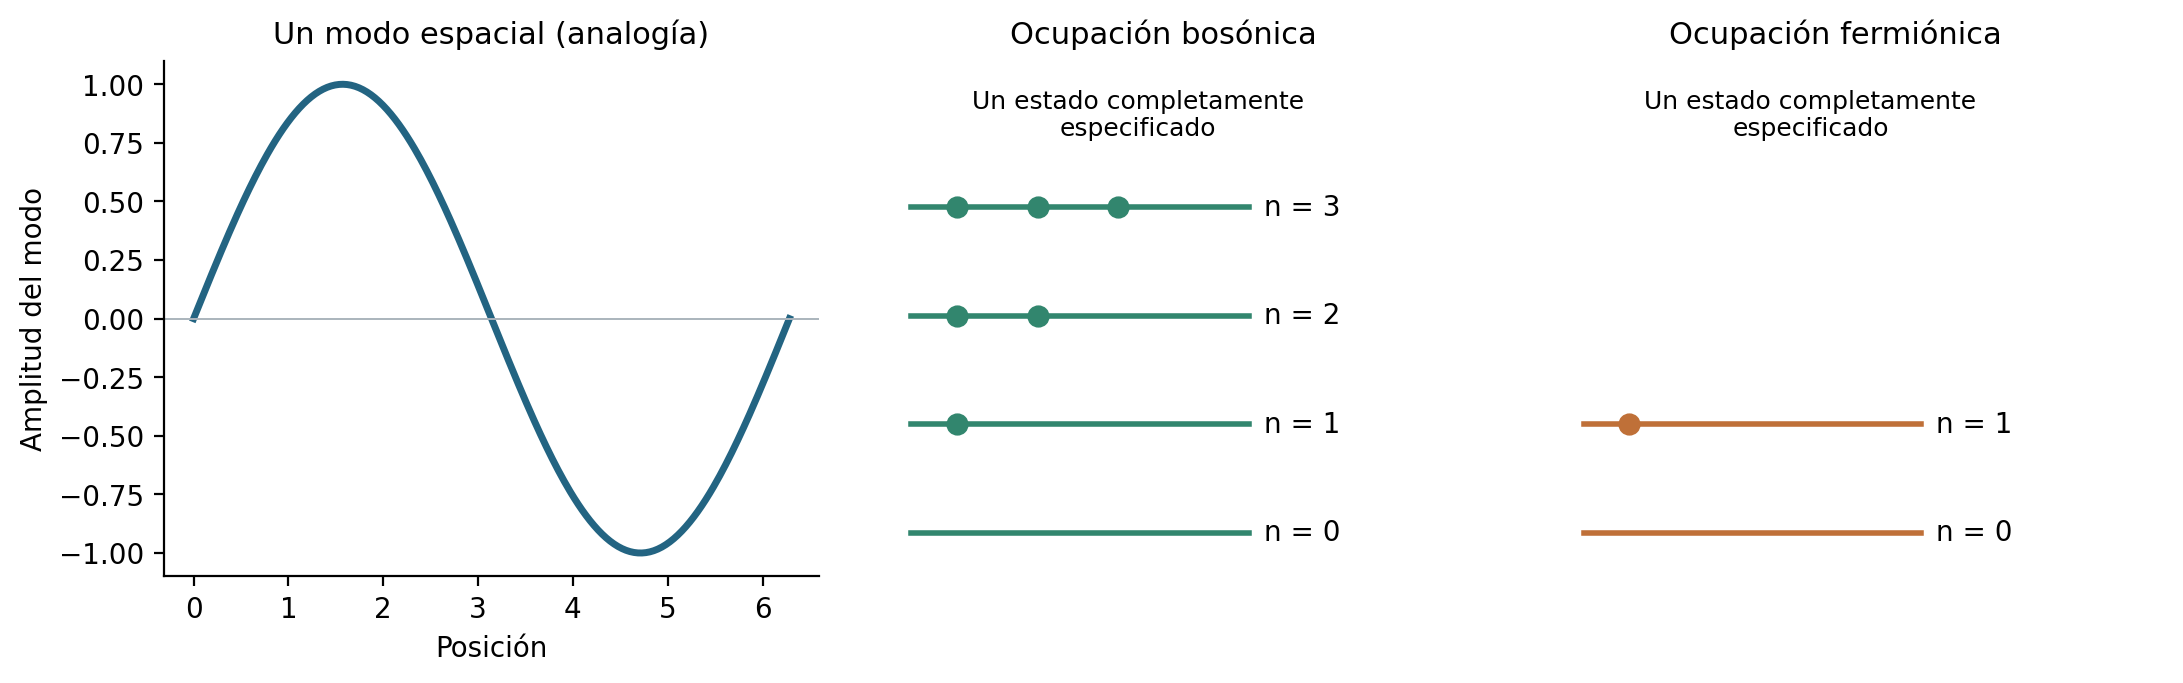
\includegraphics[width=1\linewidth,height=\textheight,keepaspectratio,alt={Figura E.1. Un perfil espacial y dos reglas de ocupación de un estado cuántico. Para un estado bosónico pueden existir muchas ocupaciones; para un estado fermiónico completamente especificado, incluidos sus índices internos, sólo 0 o 1. La onda dibujada sirve de analogía de un modo; no es la trayectoria de una bolita ni una imagen literal del campo electrónico.}]{../figuras/E_01_campos_ocupacion.png}
\caption{Figura E.1. Un perfil espacial y dos reglas de ocupación de un
estado cuántico. Para un estado bosónico pueden existir muchas
ocupaciones; para un estado fermiónico completamente especificado,
incluidos sus índices internos, sólo 0 o 1. La onda dibujada sirve de
analogía de un modo; no es la trayectoria de una bolita ni una imagen
literal del campo electrónico.}
\end{figure}

La masa relaciona energía y momento de una partícula libre mediante

\[
E^2=p^2c^2+m^2c^4.
\tag{E.1}
\]

La carga eléctrica determina cómo participa en la interacción
electromagnética. El espín describe cómo transforma su estado bajo
rotaciones: es momento angular intrínseco, no una esfera girando sobre
sí misma. Para un electrón, \(s=1/2\) y una medición de \(S_z\) produce
\(\pm\hbar/2\); esos resultados no cambian el valor de \(s\). El momento
angular orbital es otro grado de libertad {[}T2{]}.

Masa y espín clasifican cómo se transforman excitaciones libres bajo
simetrías del espacio-tiempo; las cargas describen su respuesta a
simetrías e interacciones internas. Esta organización responde al tipo
de ecuaciones que podemos construir, no a la imagen de bolitas con
propiedades pegadas.

\textbf{Masa, carga y espín no bastan para describir todo.} También
hacen falta el estado de movimiento, la ocupación, correlaciones y otros
números cuánticos. Por ejemplo, los quarks tienen carga de color y
participan en la interacción fuerte; los leptones no tienen esa carga.
El Modelo Estándar organiza los campos elementales conocidos y sus
interacciones electromagnética, débil y fuerte {[}P{]}.

{\def\LTcaptype{none} % do not increment counter
\begin{longtable}[]{@{}
  >{\raggedright\arraybackslash}p{(\linewidth - 8\tabcolsep) * \real{0.2000}}
  >{\raggedright\arraybackslash}p{(\linewidth - 8\tabcolsep) * \real{0.2000}}
  >{\raggedright\arraybackslash}p{(\linewidth - 8\tabcolsep) * \real{0.2000}}
  >{\raggedright\arraybackslash}p{(\linewidth - 8\tabcolsep) * \real{0.2000}}
  >{\raggedright\arraybackslash}p{(\linewidth - 8\tabcolsep) * \real{0.2000}}@{}}
\toprule\noalign{}
\begin{minipage}[b]{\linewidth}\raggedright
Familia elemental
\end{minipage} & \begin{minipage}[b]{\linewidth}\raggedright
Dos ejemplos
\end{minipage} & \begin{minipage}[b]{\linewidth}\raggedright
Carga eléctrica en unidades de \(e>0\)
\end{minipage} & \begin{minipage}[b]{\linewidth}\raggedright
Espín
\end{minipage} & \begin{minipage}[b]{\linewidth}\raggedright
Qué distingue a la familia
\end{minipage} \\
\midrule\noalign{}
\endhead
\bottomrule\noalign{}
\endlastfoot
Quarks, fermiones & up \(u\), down \(d\) & \(+2/3\), \(-1/3\) & \(1/2\)
& Tienen color; forman hadrones compuestos \\
Leptones, fermiones & electrón \(e^-\), neutrino electrónico \(\nu_e\) &
\(-1\), \(0\) & \(1/2\) & Sin color; el electrón también participa
electromagnéticamente \\
Bosones de calibre & fotón \(\gamma\), \(W^+\) & \(0\), \(+1\) & \(1\) &
Asociados a interacciones electromagnética y débil \\
Bosón escalar & Higgs \(H\) & \(0\) & \(0\) & Excitación del campo de
Higgs \\
\end{longtable}
}

Quarks y leptones son subfamilias de fermiones; ``bosón'' es una
clasificación por espín y estadística. También existen bosones
compuestos, por lo que la palabra no significa necesariamente elemental.
Hay tres generaciones de fermiones; la tabla muestra sólo ejemplos, no
el inventario completo. El protón y el neutrón son compuestos. Un fonón
es una excitación colectiva de un sólido, no una nueva partícula
elemental de esta tabla {[}P, CERN{]}.

El mecanismo de Higgs permite masas de fermiones cargados y de \(W/Z\)
dentro de la teoría; no significa que toda la masa de un protón sea la
suma de masas de sus quarks. Gran parte corresponde a la dinámica de
quarks y gluones. Tampoco se identifica masa con carga eléctrica: pueden
existir partículas masivas neutras. La gravedad no está incluida en el
Modelo Estándar y la materia oscura no está identificada por él; las
masas de neutrinos requieren extender su versión mínima. Éste es un
marco extraordinariamente exitoso, no una teoría final de todo {[}H,
CERN{]}.

\subsection{E.1.2. Problema resuelto: qué dice y qué no dice una
composición}\label{e.1.2.-problema-resuelto-quuxe9-dice-y-quuxe9-no-dice-una-composiciuxf3n}

\textbf{Problema.} A partir del contenido de quarks de valencia \(uud\)
del protón y \(udd\) del neutrón, y las cargas de la tabla, obtener la
carga de ambos y de un átomo de hidrógeno. Decidir si también puede
obtenerse su masa y espín sumando las etiquetas de los constituyentes.

\textbf{Paso 1: carga.} Es aditiva:

\[
Q_p/e=2(2/3)-1/3=1,\qquad
Q_n/e=2/3-2(1/3)=0,\qquad
Q_{\rm H}=Q_p-e=0.
\tag{E.2}
\]

\textbf{Paso 2: masa.} La neutralidad del neutrón no implica masa nula.
La energía interna y las interacciones contribuyen a la masa del
sistema. La operación ``sumar cargas'' no se traslada sin cambios a la
masa.

\textbf{Paso 3: espín.} Tres números \(1/2\) no autorizan a asignar
\(3/2\) al protón. Los momentos angulares se acoplan y la estructura
interna importa. Las etiquetas de los constituyentes restringen los
estados posibles, pero no seleccionan por sí solas el estado compuesto
observado.

\textbf{Lectura para el detector.} Se puede estudiar un fonón como
cuanto de un modo colectivo sin resolver de nuevo los quarks de cada
núcleo. La elección de variables efectivas aprovecha una separación de
escalas; no contradice la descripción más fundamental.

\subsection{E.1.3. Actividad evaluada}\label{e.1.3.-actividad-evaluada}

\textbf{E01.1 --- Clasificación razonada, 3 puntos.} Clasificar
electrón, fotón, protón y fonón como elemental, compuesto o colectivo.
Para dos de ellos, indicar qué información adicional a masa, carga y
espín se necesita para describir un estado concreto. Justificar por qué
``neutro'' no equivale a ``sin interacciones''.

\textbf{Respuesta E01.1:} \emph{Escribir aquí.}

\textbf{E01.2 --- Balance y límites, 4 puntos.} Un núcleo idealizado
contiene dos protones y dos neutrones, y hay tres electrones alrededor.
Obtener la carga total. Explicar por qué ese cálculo no permite obtener
automáticamente la masa ni el espín total. No se pide determinar si ese
ion sería estable.

\textbf{Respuesta E01.2:} \emph{Escribir aquí.}

\textbf{E01.3 --- Analizar una figura, 3 puntos.} En la figura E.1, un
compañero ocupa dos veces el mismo estado fermiónico porque ``pueden ser
dos electrones de espín distinto''. Precisar cuándo la afirmación es
correcta y cuándo contradice la definición de estado utilizada. Explicar
por qué un fonón no exige añadir una nueva especie al Modelo Estándar.

\textbf{Respuesta E01.3:} \emph{Escribir aquí.}

\textbf{Condición esencial:} distinguir estado de especie, y excitación
colectiva de partícula elemental. La tabla y la aritmética deben
acompañarse de esa distinción.

\subsection{E.1.4. Conexión con A--D y
fuentes}\label{e.1.4.-conexiuxf3n-con-ad-y-fuentes}

En \textbf{A.1--A.2}, espín es un índice que interviene en trazas y
normalizaciones. En \textbf{B.1--B.3}, fermiones y bosones explican
factores de ocupación diferentes. En \textbf{C.0}, el campo de orden es
una descripción colectiva, no el campo de una nueva partícula
fundamental. \textbf{D} utiliza esta separación para fijar el alcance
del modelo efectivo.

Fuentes: \href{https://home.cern/science/physics/standard-model/}{CERN,
Modelo Estándar} {[}CERN{]};
\href{https://pdg.lbl.gov/chris/museum_version/standard_model.html}{Particle
Data Group, clasificación} {[}P{]};
\href{https://www.damtp.cam.ac.uk/user/tong/qft/qfthtml/S0.html}{D.
Tong, introducción a campos} {[}T1{]};
\href{https://www.damtp.cam.ac.uk/user/tong/pp/pp2.pdf}{D. Tong,
partículas y espín} {[}T2{]};
\href{https://home.cern/sites/default/files/file/scientists/CCJulAug17_HIGSAT5.pdf}{CERN,
cinco años del Higgs y masa compuesta} {[}H{]}. Las analogías y el
problema resuelto son construcciones de este cuaderno.

\newpage

\section{E.2. Nambu y espín: dos índices
distintos}\label{e.2.-nambu-y-espuxedn-dos-uxedndices-distintos}

\textbf{ID E02 · Estado: ABIERTO · Objetivo:} construir la matriz Nambu
por espín de un singlete sencillo, interpretar su traza y explicar por
qué duplicar componentes no duplica los electrones físicos.

\subsection{E.2.1. Introducción: una tabla con dos
índices}\label{e.2.1.-introducciuxf3n-una-tabla-con-dos-uxedndices}

Una matriz puede organizar simultáneamente dos clasificaciones. En
circuitos, un vector puede llevar un índice de nodo y otro de
componente; cuatro entradas no significan cuatro circuitos completos.
Aquí el índice de espín tiene dos componentes y Nambu organiza
operadores de destrucción y creación. La combinación es un producto
tensorial de dos espacios de dimensión dos.

En una base adaptada a inversión temporal, compatible con el singlete
utilizado en A, se escribe

\[
\Psi_{\mathbf k}=\begin{pmatrix}
c_{\mathbf k\uparrow}\\c_{\mathbf k\downarrow}\\
c^\dagger_{-\mathbf k\downarrow}\\-c^\dagger_{-\mathbf k\uparrow}
\end{pmatrix}.
\tag{E.3}
\]

Los operadores \(c\) destruyen electrones y \(c^\dagger\) los crean. El
sector inferior es
\(i\sigma_y(c^\dagger_{-\mathbf k\uparrow},c^\dagger_{-\mathbf k\downarrow})^T=(c^\dagger_{-\mathbf k\downarrow},-c^\dagger_{-\mathbf k\uparrow})^T\).
Esta elección convierte la estructura singlete en una identidad de espín
en la base utilizada. Las dos entradas inferiores usan el par
relacionado por inversión temporal, con un signo convencional. No son
dos nuevas especies de antipartículas. Otra base puede cambiar los
signos y colocar \(i\sigma_y\) en el término de emparejamiento; los
resultados físicos no cambian al transformar consistentemente toda la
matriz {[}N, A{]}.

\begin{figure}
\centering
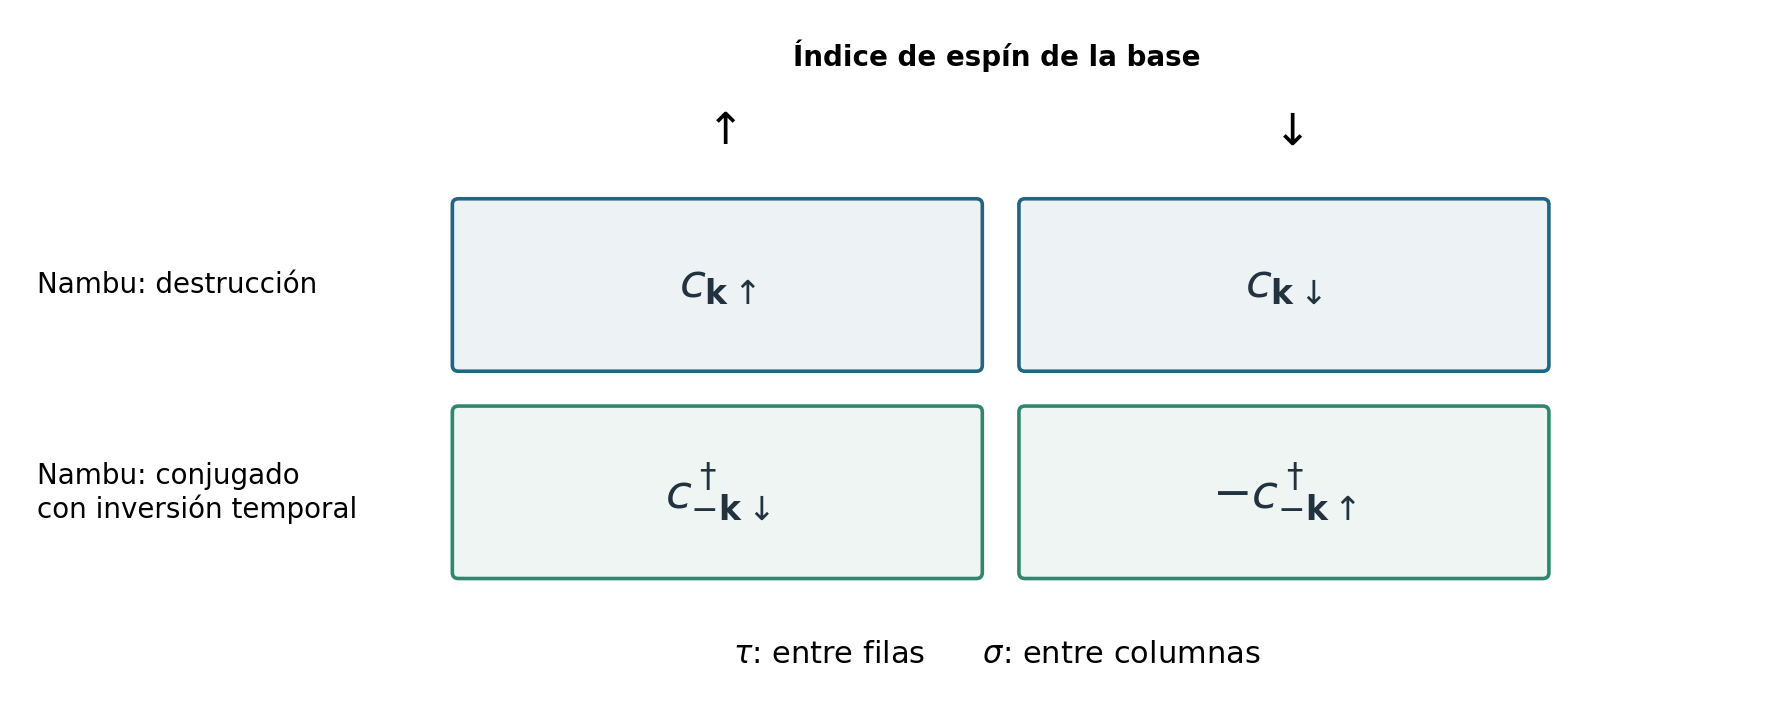
\includegraphics[width=0.92\linewidth,height=\textheight,keepaspectratio,alt={Figura E.2. Las cuatro entradas de una base Nambu por espín. Las filas distinguen destrucción y sector conjugado; las columnas, los dos índices de espín de la base elegida. Las matrices tau actúan entre filas y sigma entre columnas. El bloque conjugado invierte orden y signo de forma explícita; no se añaden cuatro electrones independientes.}]{../figuras/E_02_nambu_spin.png}
\caption{Figura E.2. Las cuatro entradas de una base Nambu por espín.
Las filas distinguen destrucción y sector conjugado; las columnas, los
dos índices de espín de la base elegida. Las matrices tau actúan entre
filas y sigma entre columnas. El bloque conjugado invierte orden y signo
de forma explícita; no se añaden cuatro electrones independientes.}
\end{figure}

Para una banda independiente del espín, sin acoplamiento espín--órbita
ni campo magnético de espín, sin superflujo (\(q=0\)), con
\(\xi_{-\mathbf k}=\xi_{\mathbf k}\) y \(\Delta\) real,

\[
H_{\rm BdG}=(\xi_{\mathbf k}\tau_3+\Delta\tau_1)\otimes\sigma_0,
\qquad \xi_{\mathbf k}=\varepsilon_{\mathbf k}-\mu.
\tag{E.4}
\]

\(\tau_i\) y \(\sigma_i\) son matrices de Pauli en espacios diferentes.
Por ejemplo, \(\tau_3\otimes\sigma_0\) distingue los dos sectores Nambu;
\(\tau_0\otimes\sigma_3\) distingue los dos índices de espín. La
representación BdG completa tiene redundancia electrón--hueco: energías
positivas y negativas están relacionadas. El prefactor \(1/2\) al
escribir un Hamiltoniano cuadrático completo, sumando todo el espacio de
momentos, en la base duplicada evita contar la misma física dos veces;
los términos constantes deben conservarse cuando se calcula energía
{[}N{]}.

\subsection{E.2.2. Problema resuelto: diagonalizar y
contar}\label{e.2.2.-problema-resuelto-diagonalizar-y-contar}

\textbf{Problema.} En unidades arbitrarias de energía, usar \(\xi=3\),
\(\Delta=4\). Encontrar la energía positiva y los pesos Nambu; después
calcular \(\operatorname{tr}_{N,s}(\tau_3\hat g)\) para
\(\hat g=(c\tau_3+s\tau_1)\otimes\sigma_0\).

El bloque de un par es

\[
\begin{pmatrix}3&4\\4&-3\end{pmatrix}
\begin{pmatrix}u\\v\end{pmatrix}
=E\begin{pmatrix}u\\v\end{pmatrix},\qquad
E^2=3^2+4^2=25.
\tag{E.5}
\]

Para \(E=5\), la primera fila exige \(v=u/2\). La normalización
\(|u|^2+|v|^2=1\) da \(|u|^2=4/5\), \(|v|^2=1/5\). Se trata de una
mezcla coherente de amplitudes; no de una moneda que escoge dos
partículas clásicas independientes.

Dentro de una traza sobre ambos espacios, la abreviatura \(\tau_i\)
significa \(\tau_i\otimes\sigma_0\). Para la traza se usa
\(\operatorname{tr}_N\tau_i\tau_j=2\delta_{ij}\) y
\(\operatorname{tr}_s\sigma_0=2\):

\[
\operatorname{tr}_{N,s}(\tau_3\hat g)
=\big(c\operatorname{tr}_N\tau_3^2+s\operatorname{tr}_N\tau_3\tau_1\big)
\operatorname{tr}_s\sigma_0=4c.
\tag{E.6}
\]

El cuatro procede de la traza en ambos espacios. No puede añadirse de
nuevo como ``cuatro partículas'' al integrar una DOS que ya incorpore
convenciones de espín y excitaciones. Ésta es la operación concreta
usada al reducir el funcional de A.

\subsection{E.2.3. Actividad evaluada}\label{e.2.3.-actividad-evaluada}

\textbf{E02.1 --- Cálculo, 4 puntos.} Repetir la diagonalización para
\(\xi=5\) y \(\Delta=12\) en las mismas unidades. Dar ambas energías y
los pesos normalizados de la rama positiva. Mostrar al menos una
verificación con la matriz original.

\textbf{Respuesta E02.1:} \emph{Escribir aquí.}

\textbf{E02.2 --- Índices, 3 puntos.} Calcular las matrices diagonales
\(\tau_3\otimes\sigma_0\) y \(\tau_0\otimes\sigma_3\) en la base E.3.
Indicar qué parejas de entradas diferencia cada una. Explicar el
significado del signo de la cuarta componente.

\textbf{Respuesta E02.2:} \emph{Escribir aquí.}

\textbf{E02.3 --- Auditoría de un argumento, 3 puntos.} Un cálculo usa
\(N_0\) por espín, toma una traza Nambu/espín completa y después
multiplica todo por cuatro ``porque hay cuatro partículas en el
espinor''. Identificar qué comprobaciones de normalización exigirías y
por qué esa justificación es incorrecta. No se pide adivinar el
prefactor final sin conocer la definición de la integral.

\textbf{Respuesta E02.3:} \emph{Escribir aquí.}

\textbf{Condición esencial:} reconocer la redundancia Nambu y mantener
separados los espacios de espín y Nambu. No interpretar los huecos de
esta base como positrones libres.

\subsection{E.2.4. Conexión con A--D y
fuentes}\label{e.2.4.-conexiuxf3n-con-ad-y-fuentes}

\textbf{A.2.2, A.6b--A.6d:} base, trazas y gradiente covariante.
\textbf{B.2:} el espectro anómalo lleva información de coherencia que la
DOS por sí sola no contiene. \textbf{C.0:} la fase y amplitud del
condensado corresponden a una descripción colectiva derivada; no son
componentes del espín. \textbf{D:} la normalización debe conservarse al
trasladar resultados entre capas.

Fuentes: \href{https://topocondmat.org/test/w1_topointro/0d.html}{curso
de TU Delft, representación BdG y redundancia} {[}N{]};
\href{https://arxiv.org/pdf/1909.00992v1}{Virtanen et al., expresión
quasiclásica}, ecuación (20) {[}A{]}. La base de E.3 es la adaptación
explícita usada aquí; no se copian sin transformar signos de bases
diferentes. La diagonalización y el cálculo de trazas anteriores son
ejercicios originales de esta revisión.

\newpage

\section{E.3. Variaciones, funcionales y teorema de la
envolvente}\label{e.3.-variaciones-funcionales-y-teorema-de-la-envolvente}

\textbf{ID E03 · Estado: ABIERTO · Objetivo:} calcular una primera
variación con condiciones de borde y distinguir variar un campo de
eliminar una variable estacionaria.

\subsection{E.3.1. Introducción: una coordenada en cada
punto}\label{e.3.1.-introducciuxf3n-una-coordenada-en-cada-punto}

Una función \(F(y)\) recibe números. Un funcional \(\mathcal F[y]\)
recibe una función completa y devuelve un número. En mecánica
lagrangiana ya aparece un ejemplo: la acción recibe una trayectoria. La
energía de una cuerda deformada recibe su perfil espacial. La derivada
funcional responde cuánto cambia el resultado si se modifica el perfil
cerca de cada posición.

En una malla con coordenadas \(y_1,\ldots,y_N\), la energía es una
función de \(N\) variables. El continuo organiza sus derivadas como una
densidad:

\[
\delta\mathcal F[y;\eta]
=\left.\frac{d}{d\epsilon}\mathcal F[y+\epsilon\eta]\right|_{\epsilon=0}
=\int\frac{\delta\mathcal F}{\delta y(x)}\eta(x)\,dx,
\tag{E.7}
\]

con los términos de borde tratados según las variaciones permitidas.
\(\eta\) es una dirección de prueba; \(\epsilon\) controla su tamaño.
\(\delta\mathcal F/\delta y\) no es la energía ni la derivada de una
curva de equilibrio, sino el coeficiente de cada perturbación local.

\begin{figure}
\centering
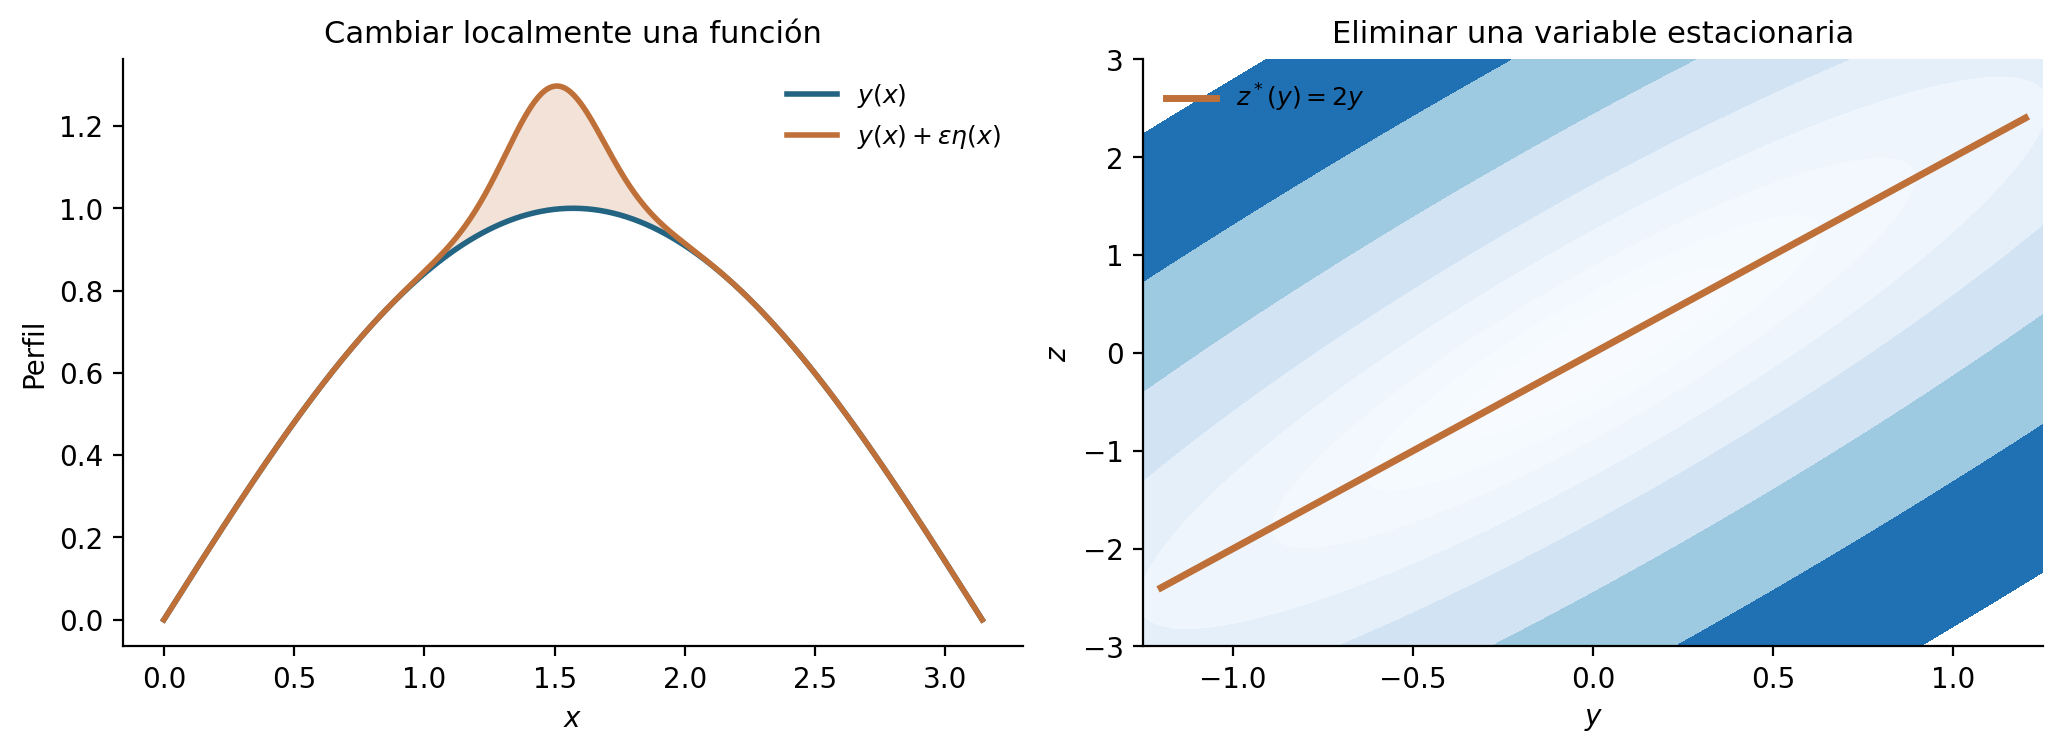
\includegraphics[width=0.87\linewidth,height=\textheight,keepaspectratio,alt={Figura E.3. Izquierda: un perfil y una perturbación local admisible. Derecha: la variable interna z se acomoda en el valle z=2y de una energía de dos variables. Seguir el valle ilustra eliminar una variable estacionaria; la pendiente y la curvatura deben distinguirse.}]{../figuras/E_03_variacion_envolvente.png}
\caption{Figura E.3. Izquierda: un perfil y una perturbación local
admisible. Derecha: la variable interna z se acomoda en el valle z=2y de
una energía de dos variables. Seguir el valle ilustra eliminar una
variable estacionaria; la pendiente y la curvatura deben distinguirse.}
\end{figure}

\subsection{E.3.2. Problema resuelto: perfil estático y variable
eliminada}\label{e.3.2.-problema-resuelto-perfil-estuxe1tico-y-variable-eliminada}

\textbf{Parte I: funcional.} En unidades adimensionales y con extremos
fijos \(y(0)=y(\pi)=0\), considerar

\[
\mathcal F[y]=\int_0^\pi\left[\frac{(y')^2}{2}+\frac{y^2}{2}-2y\sin x\right]dx.
\tag{E.8}
\]

Insertar \(y+\epsilon\eta\) y conservar términos lineales produce

\[
\begin{aligned}
\delta\mathcal F&=\int_0^\pi[y'\eta'+y\eta-2\sin x\,\eta]dx\\
&=[y'\eta]_0^\pi+\int_0^\pi[-y''+y-2\sin x]\eta\,dx.
\end{aligned}\tag{E.9}
\]

Como los extremos de \(y\) están fijados, \(\eta(0)=\eta(\pi)=0\):
desaparece el término de borde. La arbitrariedad de \(\eta\) da
\(-y''+y=2\sin x\). La solución \(y=\sin x\) satisface ecuación y
fronteras. Además, \(\delta^2\mathcal F=\int[(\eta')^2+\eta^2]dx>0\)
para toda perturbación no nula: aquí el estacionario es un mínimo. La
primera variación nula por sí sola no habría demostrado esa estabilidad.

Si los extremos fuesen libres, no se puede borrar el término de borde
por costumbre. Para este funcional, la condición natural sería \(y'=0\)
en esos extremos. Es la misma lógica que distingue imponer un
desplazamiento e imponer una fuerza en mecánica.

\textbf{Parte II: envolvente.} Considérese ahora la función ordinaria

\[
F(y,z)=\frac{y^2}{2}+\frac{(z-2y)^2}{2}.
\tag{E.10}
\]

La condición interna \(F_z=z-2y=0\) da \(z^*(y)=2y\). La función
reducida es \(\bar F(y)=F(y,z^*(y))=y^2/2\). Por regla de la cadena,

\[
\frac{d\bar F}{dy}=F_y+F_z\frac{dz^*}{dy}
=y-2(z^*-2y)+0=y.
\tag{E.11}
\]

El término de la derivada de \(z^*\) desaparece porque multiplica
\(F_z=0\), no porque \(z^*\) sea constante. Es la forma de la envolvente
que utiliza A.2.3: los ángulos espectrales ya satisfacen su ecuación,
mientras la amplitud todavía puede variar.

\textbf{Una precaución de segundo orden.} No se debe congelar otra vez
la variable al calcular una segunda derivada. En este ejemplo
\(F_{yy}=5\) a \(z\) fijo, pero \(\bar F''=1\). Para una variable
interna no degenerada,

\[
\bar F''=F_{yy}-\frac{F_{yz}^2}{F_{zz}}=5-\frac{(-2)^2}{1}=1.
\tag{E.12}
\]

La relajación interna reduce aquí la rigidez. Esto importa para
capacidades y estabilidad: una identidad de primeras derivadas no
autoriza a omitir la respuesta espectral en todas las derivadas
posteriores. En un extremo degenerado o un cambio de rama se deben
revisar las hipótesis de diferenciabilidad.

\subsection{E.3.3. Actividad evaluada}\label{e.3.3.-actividad-evaluada}

\textbf{E03.1 --- Variación y fronteras, 4 puntos.} Para

\[
\mathcal G[y]=\int_0^\pi\left[(y')^2+\frac{y^2}{2}-3y\sin x\right]dx,
\qquad y(0)=y(\pi)=0,
\tag{E.13}
\]

obtener la primera variación, conservar el término de borde antes de
usar las condiciones y encontrar una solución proporcional a \(\sin x\).
Explicar si el estacionario es estable mediante la segunda variación.

\textbf{Respuesta E03.1:} \emph{Escribir aquí.}

\textbf{E03.2 --- Error de eliminación, 3 puntos.} Para
\(H(y,z)=y^2+(z-3y)^2/2\), encontrar \(z^*(y)\) y comparar
\(dH(y,z^*)/dy\) con la derivada a \(z\) fijo evaluada en esa rama.
Después repetir la comparación cuando alguien utiliza por error
\(z=3y+0.1\). Indicar cuál hipótesis del teorema dejó de cumplirse.

\textbf{Respuesta E03.2:} \emph{Escribir aquí.}

\textbf{E03.3 --- Lectura física, 3 puntos.} Explicar por qué se pueden
eliminar los ángulos estacionarios de A sin imponer \(G=0\) durante todo
un evento. Indicar qué cantidad adicional se necesita para convertir la
pendiente de energía en una velocidad de evolución. Usar la figura E.3
para justificar la diferencia entre pendiente y rigidez.

\textbf{Respuesta E03.3:} \emph{Escribir aquí.}

\textbf{Condición esencial:} no eliminar términos de borde sin
justificarlo y no confundir la estacionariedad espectral con el
equilibrio instantáneo de la amplitud.

\subsection{E.3.4. Conexión con A--D y
fuentes}\label{e.3.4.-conexiuxf3n-con-ad-y-fuentes}

\textbf{A.2.3, A.8a--A.8b:} aplican la variación y la envolvente a
\href{https://arxiv.org/pdf/1909.00992v1}{Virtanen et al., ecuación
(20)}. \textbf{B.5 y B.11:} fijar espectro u ocupaciones produce
derivadas distintas. \textbf{C.1--C.4:} fuerzas, movilidad y trabajo
completan la dinámica. \textbf{D:} las identidades prueban coherencia
interna, no validación experimental. Los ejemplos E.7--E.13 se derivan
aquí.

\newpage

\section{E.4. Electrones y huecos: del diodo al
superconductor}\label{e.4.-electrones-y-huecos-del-diodo-al-superconductor}

\textbf{ID E04 · Estado: ABIERTO · Objetivo:} calcular carga y energía
respecto de una referencia ocupada y distinguir un hueco de
semiconductor, una antipartícula y una componente Nambu.

\subsection{E.4.1. Introducción: llevar la cuenta de lo que
falta}\label{e.4.1.-introducciuxf3n-llevar-la-cuenta-de-lo-que-falta}

En un semiconductor, describir por separado todos los electrones de una
banda casi llena resulta poco práctico. Se elige la banda llena como
referencia y se sigue la escasa población de vacantes. Si un electrón
ocupa la vacante vecina, la vacante se desplaza en sentido contrario. Es
una nueva contabilidad del mismo sistema electrónico {[}M1{]}.

En un diodo se comparan poblaciones de electrones de conducción y huecos
de valencia. En equilibrio, difusión y arrastre por el campo de la unión
se compensan; eso no significa que cada portador esté inmóvil. Bajo
polarización cambian las poblaciones y aparecen corrientes netas. El
campo y las bandas del diodo hacen familiar la elección de una
referencia, pero el gap de un semiconductor no procede del
emparejamiento de Cooper {[}M2{]}.

\begin{figure}
\centering
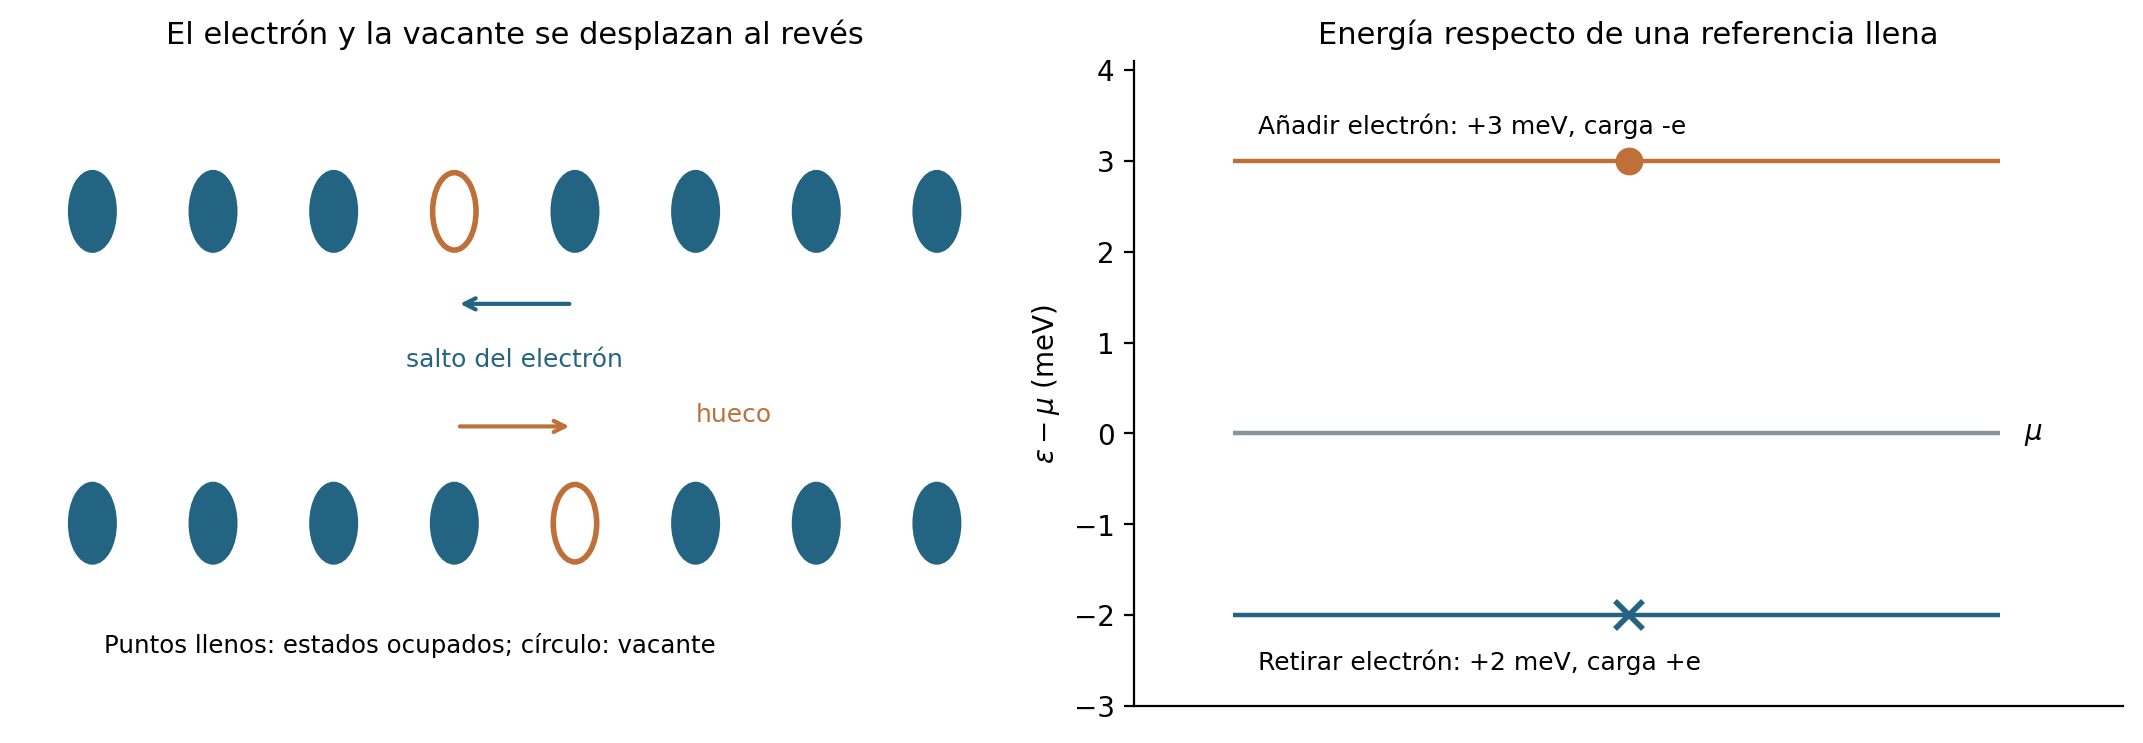
\includegraphics[width=1\linewidth,height=\textheight,keepaspectratio,alt={Figura E.4. Izquierda: un electrón ocupa una vacante vecina y el hueco efectivo se desplaza en sentido contrario. Derecha: comparación entre un electrón añadido por encima de mu y uno retirado por debajo; ambas operaciones producen excitaciones de energía positiva. Los niveles son un dibujo de contabilidad, no un perfil de bandas de un diodo real.}]{../figuras/E_04_electron_hueco.png}
\caption{Figura E.4. Izquierda: un electrón ocupa una vacante vecina y
el hueco efectivo se desplaza en sentido contrario. Derecha: comparación
entre un electrón añadido por encima de mu y uno retirado por debajo;
ambas operaciones producen excitaciones de energía positiva. Los niveles
son un dibujo de contabilidad, no un perfil de bandas de un diodo real.}
\end{figure}

Aquí ``energía de excitación'' se mide respecto del equilibrio a
potencial químico fijado: es el cambio de \(U-\mu N\). Si cambia el
número electrónico, \(\delta U=\mu\,\delta N+E_{\rm excitaciones}\); la
energía interna absoluta no se confunde con esa referencia.

Si el electrón retirado tenía energía \(\varepsilon<\mu\) y carga
\(-e\), la excitación relativa al mar lleno cambia la carga en \(+e\) y
cuesta \(\mu-\varepsilon>0\). La energía negativa relativa
\(\xi=\varepsilon-\mu\) del estado electrónico no es una energía
negativa de la excitación. En un metal normal, cerca de la superficie de
Fermi, se puede llevar esta cuenta separando electrones añadidos y
vacantes.

En superconductividad, la excitación mezcla ambos canales. Para un
bloque BCS uniforme, \(E=\sqrt{\xi^2+|\Delta|^2}\) y

\[
|u|^2=\frac12\left(1+\frac{\xi}{E}\right),\qquad
|v|^2=\frac12\left(1-\frac{\xi}{E}\right).
\tag{E.14}
\]

En la contabilidad de carga electrónica de ese modo,
\(Q_{\rm qp}=-e(|u|^2-|v|^2)=-e\xi/E\). Es una expectativa de carga
relativa de la excitación, no una nueva especie con carga fundamental
fraccionaria. El condensado y la respuesta de pantalla completan la
conservación eléctrica del sistema. En \(\xi=0\), los dos pesos son
iguales: una excitación puede contener energía aun cuando esa
expectativa de carga se anule {[}N{]}.

El hueco de un sólido no es un positrón: requiere una referencia
electrónica ocupada y propiedades de banda. La componente conjugada de
Nambu tampoco añade una banda de valencia física. Es una organización
útil para escribir el emparejamiento. Simetría electrón--hueco y
ausencia de desequilibrio de carga son hipótesis de un sector cinético;
no obligan a que la población sea térmica ni a que no exista una
corriente superconductora.

\subsection{E.4.2. Problema resuelto: energía positiva con carga neta
nula}\label{e.4.2.-problema-resuelto-energuxeda-positiva-con-carga-neta-nula}

\textbf{Problema.} Con referencia al estado ocupado a \(T=0\), añadir un
electrón a \(\mu+3\) meV y retirar otro de \(\mu-2\) meV. Obtener número
neto de electrones, carga y energía de excitación. Después compararlo
con una cuasipartícula BCS en \(\xi=0\).

La primera operación aporta \(\delta N=+1\), \(\delta Q=-e\) y 3 meV. La
segunda aporta \(\delta N=-1\), \(\delta Q=+e\) y 2 meV. Por tanto,

\[
\delta N_{\rm total}=0,\qquad \delta Q_{\rm total}=0,
\qquad E_{\rm excitaciones}=5\,\mathrm{meV}.
\tag{E.15}
\]

Un calorímetro puede registrar la energía aunque no se haya inyectado
carga neta. Dos poblaciones de energías diferentes pueden mantener esa
neutralidad. La misma distinción es importante al absorber un fotón en
un sólido.

Para una cuasipartícula BCS con \(\xi=0\), E.14 da \(|u|^2=|v|^2=1/2\) y
\(E=|\Delta|\). Aquí hay una superposición coherente dentro del modo; no
es el mismo estado que dos excitaciones normales clásicamente separadas.
La coincidencia de carga neta no identifica los dos estados.

\subsection{E.4.3. Actividad evaluada}\label{e.4.3.-actividad-evaluada}

\textbf{E04.1 --- Contabilidad, 4 puntos.} Añadir un electrón a
\(\mu+4\) meV y retirar dos electrones, uno a \(\mu-1\) meV y otro a
\(\mu-2\) meV. Obtener \(\delta N\), \(\delta Q\) y energía total de
excitación. Explicar por qué no se suman los valores de \(\xi\) con sus
signos para obtener esa energía.

\textbf{Respuesta E04.1:} \emph{Escribir aquí.}

\textbf{E04.2 --- Analizar el dibujo, 3 puntos.} Si la vacante del panel
izquierdo se mueve a la derecha, indicar el sentido del salto
electrónico y el sentido de corriente convencional asociado a ese salto.
Explicar qué parte de esta analogía sirve para la unión p--n y qué parte
no basta para describir una cuasipartícula superconductora.

\textbf{Respuesta E04.2:} \emph{Escribir aquí.}

\textbf{E04.3 --- Separar conceptos, 3 puntos.} Evaluar estas
afirmaciones con una corrección breve: ``un hueco es un positrón dentro
del metal''; ``energía de excitaciones positiva exige carga neta
distinta de cero''; ``simetría electrón--hueco permite reemplazar
cualquier distribución por Fermi--Dirac''.

\textbf{Respuesta E04.3:} \emph{Escribir aquí.}

\textbf{Condición esencial:} definir la referencia antes de asignar
signos de energía y carga, y distinguir neutralidad, coherencia y
termalidad.

\subsection{E.4.4. Conexión con A--D y
fuentes}\label{e.4.4.-conexiuxf3n-con-ad-y-fuentes}

\textbf{A.2:} la contribución normal cuenta electrones y vacantes;
explica factores que reaparecen en las energías. \textbf{B.1 y B.11:} el
sector simétrico todavía conserva distribuciones no térmicas.
\textbf{C.0--C.4:} corriente y conservación de energía son ecuaciones
relacionadas, pero distintas. \textbf{D:} una sola temperatura
equivalente no reemplaza esos balances ni todas las poblaciones.

Fuentes:
\href{https://live.ocw.mit.edu/courses/6-012-microelectronic-devices-and-circuits-fall-2009/a37c73e7fcff4bcb5c5f1177e12d0891_MIT6_012F09_lec01.pdf}{MIT
6.012, portadores en semiconductores} {[}M1{]};
\href{https://web.mit.edu/6.012/www/}{MIT 6.012, transporte y unión
p--n} {[}M2{]};
\href{https://topocondmat.org/test/w1_topointro/0d.html}{TU Delft,
representación BdG} {[}N{]}. E.14 sigue también de diagonalizar la
matriz de E.4; la contabilidad numérica es un ejemplo propio.

\newpage

\section{E.5. De modos normales a DOS y
DFPT}\label{e.5.-de-modos-normales-a-dos-y-dfpt}

\textbf{ID E05 · Estado: ABIERTO · Objetivo:} construir una DOS a partir
de modos, distinguirla de una ocupación y de un espectro ponderado de
interacción, y explicar qué calcula DFPT para alimentar B.

\subsection{E.5.1. Introducción: cuántos modos hay y cuánto
interactúan}\label{e.5.1.-introducciuxf3n-cuuxe1ntos-modos-hay-y-cuuxe1nto-interactuxfaan}

Para \(N\) masas con un desplazamiento escalar cada una, la teoría de
oscilaciones pequeñas entrega \(N\) modos normales. Escribir \(N\) modos
no implica que todos estén excitados. Los autovectores describen las
formas; los autovalores, las frecuencias; las ocupaciones indican cuánta
energía hay en cada modo. Son tres piezas distintas.

Una DOS reúne las frecuencias en una función que cuenta estados. Para
una cadena finita,

\[
F_\omega(\omega)=\sum_{\nu=1}^{N}\delta(\omega-\omega_\nu),
\qquad \int_0^\infty F_\omega(\omega)\,d\omega=N.
\tag{E.16}
\]

La delta de Dirac concentra un área de un modo. Su altura puntual no es
una población infinita. En una figura se puede reemplazar por un pico
estrecho de área conservada; ese ensanchamiento gráfico no representa
automáticamente una vida media física.

\begin{figure}
\centering
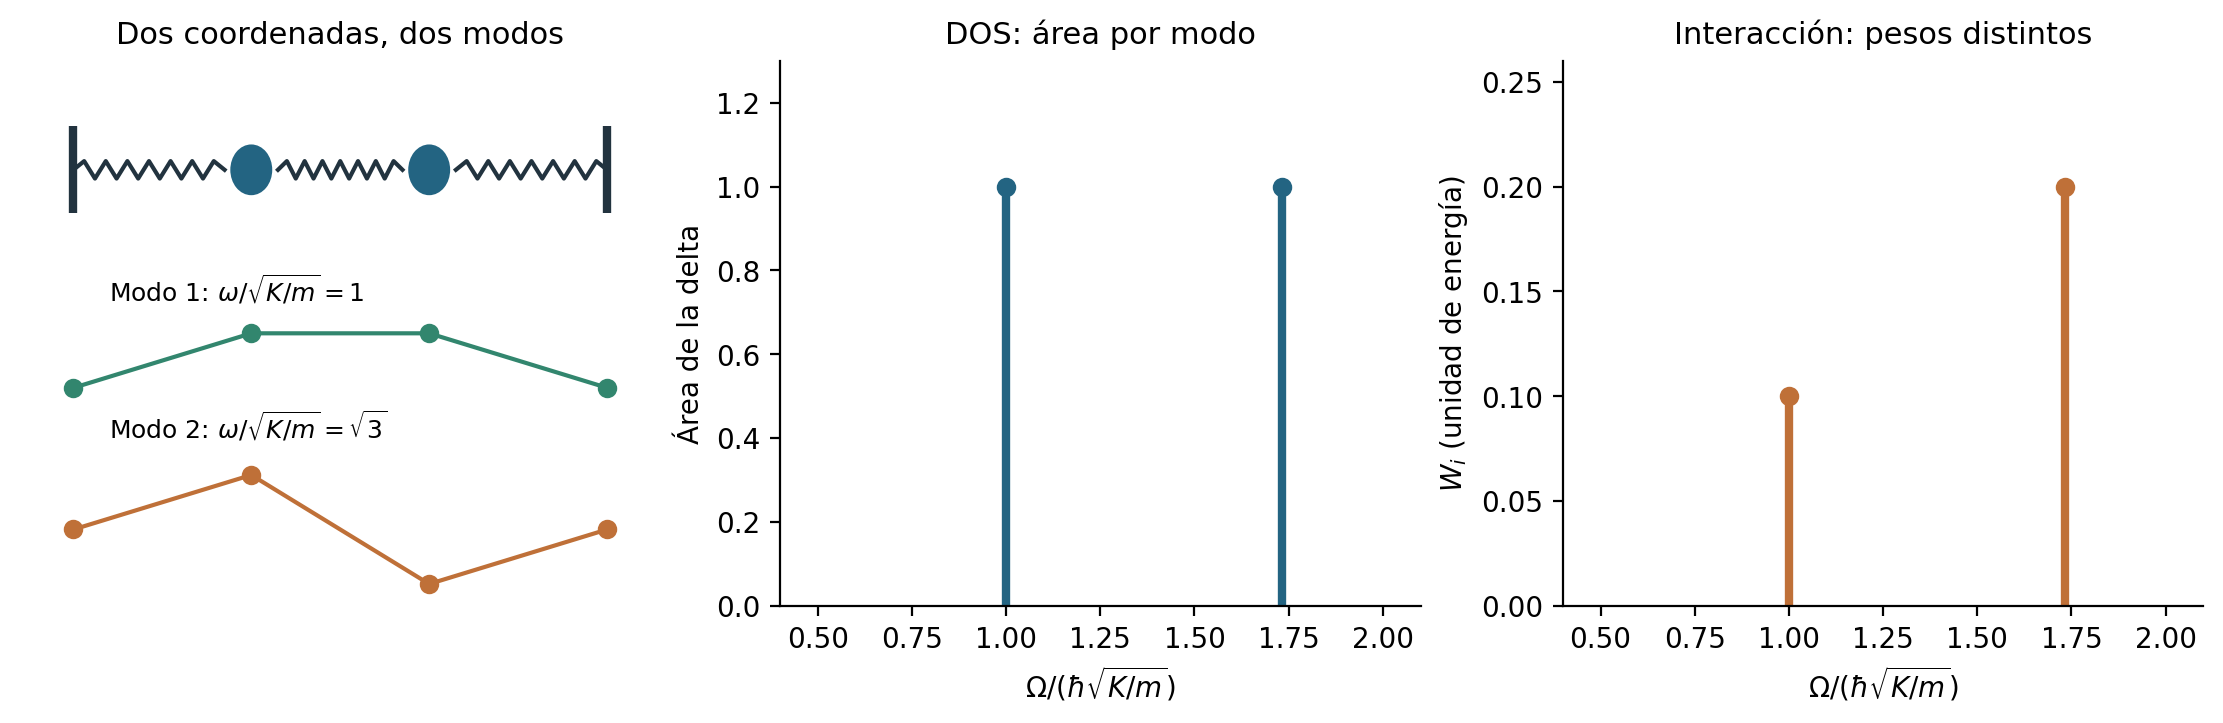
\includegraphics[width=1\linewidth,height=\textheight,keepaspectratio,alt={Figura E.5. Cadena de dos masas entre paredes y sus dos modos: en fase y en oposición. Las frecuencias alimentan dos líneas de DOS con área unitaria. Los mismos modos pueden tener pesos de acoplamiento diferentes; contar modos y medir cuánto interactúan responde a preguntas distintas.}]{../figuras/E_05_modos_dos.png}
\caption{Figura E.5. Cadena de dos masas entre paredes y sus dos modos:
en fase y en oposición. Las frecuencias alimentan dos líneas de DOS con
área unitaria. Los mismos modos pueden tener pesos de acoplamiento
diferentes; contar modos y medir cuánto interactúan responde a preguntas
distintas.}
\end{figure}

En un cristal tridimensional con \(s\) átomos por celda hay \(3s\) ramas
por vector de onda \(\mathbf q\). Una convención por celda y por energía
es

\[
F_\Omega(\Omega)=\frac{1}{N_q}\sum_{\mathbf q\nu}
\delta(\Omega-\hbar\omega_{\mathbf q\nu}),\qquad
\int F_\Omega\,d\Omega=3s.
\tag{E.17}
\]

La normalización por átomo dividiría este conteo por \(s\). Si \(N_i\)
cuenta celdas por volumen, debe multiplicar una DOS por celda; no una
DOS ya normalizada por átomo. Además,

\[
F_\Omega(\Omega)=\frac1\hbar F_\omega(\Omega/\hbar).
\tag{E.18}
\]

Cambiar el eje sin transformar la altura cambia el número de modos. Si
se usa frecuencia ordinaria \(\nu\) en THz, la energía es \(h\nu\), no
\(\hbar\nu\). La DOS electrónica normalizada \(\rho\) de A es otra
cantidad: debe multiplicarse por su escala electrónica, no por \(N_i\).

\textbf{Dónde entra DFPT.} Las frecuencias provienen de la curvatura de
la energía electrónica más iónica respecto de desplazamientos atómicos.
DFPT calcula la respuesta electrónica lineal autoconsistente a una
perturbación; con ella se obtienen constantes de fuerza y acoplamientos
electrón--fonón. Así reemplaza un resorte supuesto por una respuesta del
material calculada dentro de DFT {[}DF{]}.

\subsection{E.5.2. Problema resuelto: de resortes a entradas
materiales}\label{e.5.2.-problema-resuelto-de-resortes-a-entradas-materiales}

\textbf{Parte I: dos masas.} Dos masas iguales \(m\) están unidas por
tres resortes iguales \(K\), con paredes fijas. Para desplazamientos
\(u_1,u_2\),

\[
V=\frac K2[u_1^2+(u_2-u_1)^2+u_2^2],\qquad
m\ddot{\mathbf u}=-K\begin{pmatrix}2&-1\\-1&2\end{pmatrix}\mathbf u.
\tag{E.19}
\]

Los autovectores normalizados son \((1,1)/\sqrt2\) y \((1,-1)/\sqrt2\).
Los autovalores de la matriz adimensional son 1 y 3:
\(\omega_1=\sqrt{K/m}\) y \(\omega_2=\sqrt{3K/m}\). No aparecen cuatro
modos por tener dos masas y dos resortes exteriores; cuentan los grados
de libertad independientes.

\textbf{Parte II: población.} Elegir \(\hbar\sqrt{K/m}=1\) en una unidad
de energía. Si las ocupaciones son \(n_1=2\) y \(n_2=0\), la energía de
excitaciones es 2 unidades. La energía de punto cero se omite de esta
referencia y no cambia ese resultado. La DOS contiene dos modos antes y
después de excitar: lo que cambió fue \(n_\nu\).

\textbf{Parte III: interacción.} Como ejemplo espectral, sea

\[
\alpha^2F(\Omega)=W_1\delta(\Omega-\Omega_1)
+W_2\delta(\Omega-\Omega_2),\qquad
\lambda=2\left(\frac{W_1}{\Omega_1}+\frac{W_2}{\Omega_2}\right).
\tag{E.20}
\]

Con eje de energía y \(\alpha^2F\) adimensional, \(W_i\) tiene unidades
de energía. Si \(\Omega_1=1\), \(\Omega_2=\sqrt3\), \(W_1=0.10\) y
\(W_2=0.20\) en esa unidad, \(\lambda=0.43094\). Los pesos no son
ocupaciones ni áreas de la DOS sin ponderar. Si se duplican ambos
\(W_i\), se duplica \(\lambda\) sin cambiar las frecuencias ni el número
de modos. Este ejemplo ilustra la integral de A.32, no un ajuste de NbN.

\textbf{Parte IV: lo que sustituye al resorte en DFPT.} Cerca de una
estructura de equilibrio,

\[
E_{\rm BO}(\{u\})=E_0+\frac12\sum_{IJ}\Phi_{IJ}u_Iu_J+O(u^3),
\qquad \Phi_{IJ}=\frac{\partial^2E_{\rm BO}}{\partial u_I\partial u_J}.
\tag{E.21}
\]

\(I,J\) incluyen átomo, celda y dirección. La matriz dinámica transforma
estas curvaturas mediante las masas: \(D_{IJ}=\Phi_{IJ}/\sqrt{M_IM_J}\),
con la transformada espacial apropiada para cada \(\mathbf q\). Sus
autovalores son \(\omega^2\). No confundir esta matriz \(D_{IJ}\) con el
coeficiente escalar de difusión \(D\) de pySNSPD.

En un ejemplo electrónico no degenerado, la ecuación de respuesta tiene
la estructura

\[
(H_{\rm KS}-\varepsilon_n)\,\delta\psi_n
=-(\delta V_{\rm KS}-\delta\varepsilon_n)\psi_n.
\tag{E.22}
\]

La densidad cambia con \(\delta\psi_n\), y \(\delta V_{\rm KS}\) cambia
con esa densidad: hay que resolver la respuesta autoconsistentemente y
fijar la libertad de fase del estado. En metales y subespacios
degenerados se necesitan ocupaciones y proyectores adecuados; E.22
enseña la estructura, no es una receta completa de implementación
{[}DF{]}.

Finalmente, la perturbación del potencial proyectada sobre un modo
conecta estados electrónicos. De forma esquemática,

\[
g_{mn\nu}(\mathbf k,\mathbf q)
\sim\left\langle\psi_{m,\mathbf k+\mathbf q}\left|
\delta_{\mathbf q\nu}V_{\rm KS}\right|\psi_{n,\mathbf k}\right\rangle
\times\text{amplitud cuántica del modo}.
\tag{E.23}
\]

En E.23, \(\delta_{\mathbf q\nu}V_{\rm KS}\) designa la derivada del
potencial respecto de la coordenada normal del modo, todavía sin
multiplicar por su amplitud cuántica. Su normalización debe especificar
las masas; si la amplitud ya estuviera incluida en la perturbación, no
se multiplicaría otra vez.

El espectro \(\alpha^2F\) combina pesos \(|g|^2\), modos fonónicos y
estados electrónicos cerca del nivel de Fermi. La documentación de
PHonon define sus prefactores y normalización; E.23 sólo separa las
piezas físicas {[}QE{]}. Los factores de ocupación y coherencia
superconductora de B se aplican después: DFPT no calcula por sí sola una
cascada no térmica, una burbuja inicial ni la gTDGL del detector.

\begin{figure}
\centering
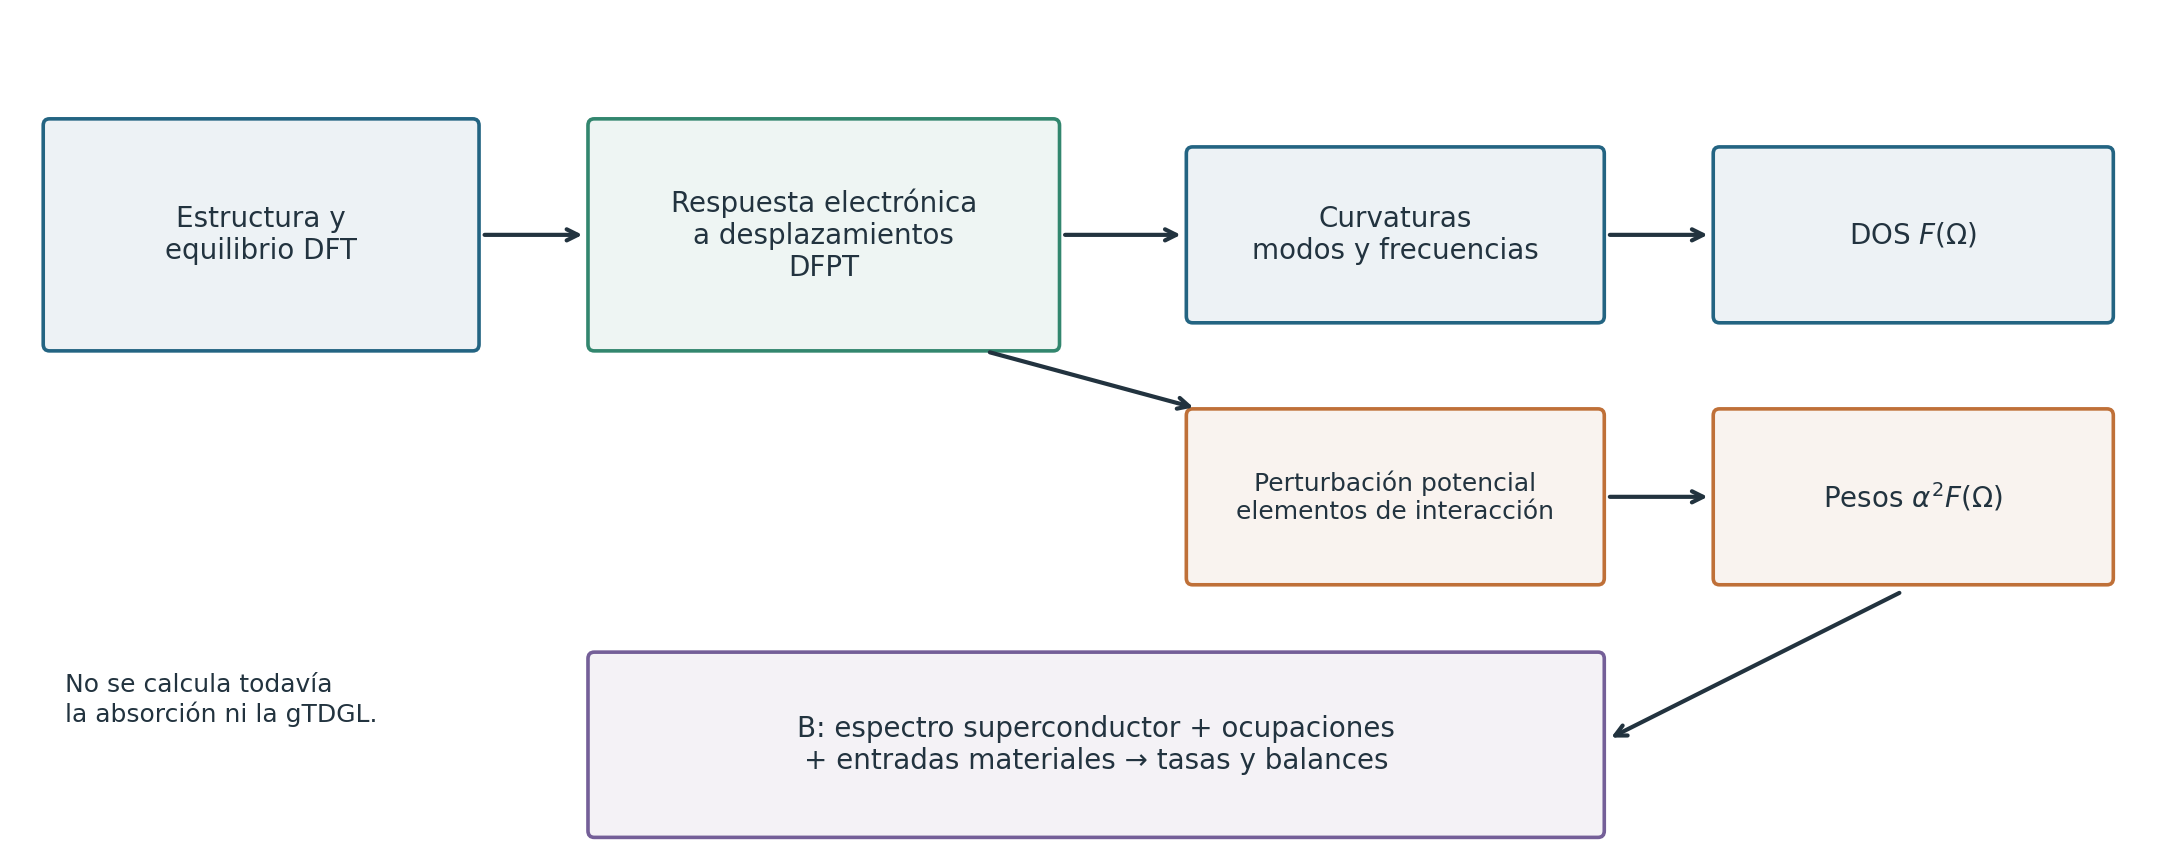
\includegraphics[width=1\linewidth,height=\textheight,keepaspectratio,alt={Figura E.6. Cadena de dependencias: estructura y respuesta electrónica producen curvaturas y elementos de interacción; de ellos se obtienen modos, DOS y espectro ponderado. B añade ocupaciones y factores de coherencia para formar tasas y balances. Las flechas muestran dependencias, no una equivalencia entre todos los objetos.}]{../figuras/E_06_dfpt_a_cinetica.png}
\caption{Figura E.6. Cadena de dependencias: estructura y respuesta
electrónica producen curvaturas y elementos de interacción; de ellos se
obtienen modos, DOS y espectro ponderado. B añade ocupaciones y factores
de coherencia para formar tasas y balances. Las flechas muestran
dependencias, no una equivalencia entre todos los objetos.}
\end{figure}

\subsection{E.5.3. Actividad evaluada}\label{e.5.3.-actividad-evaluada}

\textbf{E05.1 --- Modos y DOS, 4 puntos.} Para tres masas iguales con
cuatro resortes iguales y extremos fijos, formar la matriz de rigidez.
Sin necesidad de hallar fórmulas exactas para las tres frecuencias,
justificar cuántos modos hay y cuánto vale la integral de la DOS total.
Explicar cómo cambiaría esa integral si se normalizara por oscilador y,
por separado, por unidad de masa física de toda la cadena. Indicar las
unidades en ambos casos. Comprobar la dimensión de la matriz dinámica.

\textbf{Respuesta E05.1:} \emph{Escribir aquí.}

\textbf{E05.2 --- Interpretar resultados, 3 puntos.} Dos cálculos tienen
idénticas frecuencias y DOS fonónica, pero el segundo duplica \(|g|^2\)
para todos los procesos. Decidir qué cambia entre número de modos,
\(\alpha^2F\), \(\lambda\) y ocupación inicial de fonones. Explicar qué
información falta para predecir una potencia electrón--fonón.

\textbf{Respuesta E05.2:} \emph{Escribir aquí.}

\textbf{E05.3 --- Unidades y frontera entre métodos, 3 puntos.} Una DOS
está tabulada por celda y por THz. Describir cómo convertir tanto el eje
como los valores a una DOS por volumen y por joule, identificando la
densidad de celdas necesaria. Explicar en qué paso del esquema E.6
entran los factores de coherencia de B.2 y las ocupaciones de B.3.

\textbf{Respuesta E05.3:} \emph{Escribir aquí.}

\textbf{Condición esencial:} no confundir DOS, ocupación y peso de
interacción; conservar el número de modos al cambiar eje y
normalización.

\subsection{E.5.4. Conexión con A--D y
fuentes}\label{e.5.4.-conexiuxf3n-con-ad-y-fuentes}

\textbf{A.1 y A.5:} convenciones y significado de \(\lambda\); la
microscopía de equilibrio y la cinética deben declarar sus
aproximaciones. \textbf{B.2--B.3:} las entradas \(F\) y \(\alpha^2F\) no
sustituyen los espectros superconductores ni sus factores de ocupación.
\textbf{C:} estas tasas afectan las fuerzas y el intercambio, pero no
fijan automáticamente la movilidad de orden. \textbf{D:} la auditoría
material exige saber de qué estructura, normalización y aproximación
proviene cada tabla.

Fuentes: \href{https://arxiv.org/abs/cond-mat/0012092}{Baroni, de
Gironcoli, Dal Corso y Giannozzi, DFPT}, revisión publicada en Reviews
of Modern Physics \textbf{73}, 515 (2001) {[}DF{]};
\href{https://www.quantum-espresso.org/Doc/ph_user_guide/node19.html}{Quantum
ESPRESSO, coeficientes electrón--fonón} {[}QE{]};
\href{https://www.quantum-espresso.org/Doc/ph_user_guide/node5.html}{PHonon,
capacidades y estructura}; \href{https://arxiv.org/abs/1005.4418}{EPW,
interpolación de acoplamientos}. La cadena de masas, las DOS discretas,
sus pesos y las actividades son ejemplos originales; no se ejecutó
DFT/DFPT del material para confeccionarlos.

\section{E.6. Registro de evaluación para la siguiente
iteración}\label{e.6.-registro-de-evaluaciuxf3n-para-la-siguiente-iteraciuxf3n}

{\def\LTcaptype{none} % do not increment counter
\begin{longtable}[]{@{}
  >{\raggedright\arraybackslash}p{(\linewidth - 8\tabcolsep) * \real{0.2000}}
  >{\raggedright\arraybackslash}p{(\linewidth - 8\tabcolsep) * \real{0.2000}}
  >{\raggedright\arraybackslash}p{(\linewidth - 8\tabcolsep) * \real{0.2000}}
  >{\raggedright\arraybackslash}p{(\linewidth - 8\tabcolsep) * \real{0.2000}}
  >{\raggedright\arraybackslash}p{(\linewidth - 8\tabcolsep) * \real{0.2000}}@{}}
\toprule\noalign{}
\begin{minipage}[b]{\linewidth}\raggedright
Tema
\end{minipage} & \begin{minipage}[b]{\linewidth}\raggedright
Respuestas recibidas
\end{minipage} & \begin{minipage}[b]{\linewidth}\raggedright
Puntaje
\end{minipage} & \begin{minipage}[b]{\linewidth}\raggedright
Condición esencial
\end{minipage} & \begin{minipage}[b]{\linewidth}\raggedright
Próximo estado
\end{minipage} \\
\midrule\noalign{}
\endhead
\bottomrule\noalign{}
\endlastfoot
E01 & Pendientes & Sin evaluar & Sin evaluar & Abierto \\
E02 & Pendientes & Sin evaluar & Sin evaluar & Abierto \\
E03 & Pendientes & Sin evaluar & Sin evaluar & Abierto \\
E04 & Pendientes & Sin evaluar & Sin evaluar & Abierto \\
E05 & Pendientes & Sin evaluar & Sin evaluar & Abierto \\
\end{longtable}
}

\textbf{Comentarios de aprendizaje para la revisión 0.4:} \emph{Escribir
aquí qué explicación funcionó, qué paso quedó oscuro o qué analogía
convendría cambiar. Estos comentarios no sustituyen los ejercicios y no
afectan negativamente la evaluación.}

\textbf{Pauta de las actividades evaluadas:} pendiente de la próxima
revisión con respuestas. Se incorporará al mismo tema y conservará los
identificadores E01--E05 para poder seguir los avances sin perder
versiones anteriores.

\end{document}
